\chapter{Luminosity Measurement using Muon Barrel Trigger Primitives}
\label{ch:DT-lumi}


During Run 2, counting of muon track candidates from the CMS Level 1 trigger system, the Barrel Muon Track Finder (BMTF),
has proven to be useful for the luminosity systematics estimation due its excellent linearity and stability \cite{LUM-17-001}.
The observable used was the barrel track sorter rate integrating BMTF track candidates over the entire orbit and over one lumi section ($\sim$23 s) period.
This counter was recorded by the BRILDAQ in real time and had a statistical precision of about 0.2\% per orbit per lumi section for the Run 2 instantaneous luminosity of  $2\times10^{34}\ \text{cm}^{-2}\text{s}^{-1}$.
The  uncertainty with the BMTF tracks at the HL-LHC instantaneous luminosity of $7.5\times10^{34}\ \text{cm}^{-2}\text{s}^{-1}$
is expected to be of the order of 25\% per bunch per second, which does not provide enough precision for an online luminometer.
Below we describe an improved luminometer design based on muon trigger primitives which will be available 
from the Phase-2 back end of the barrel detector for each of the Muon Drift Tube (DT) chambers, and provides higher count rates per bunch crossing.


\section{Detector Description and Trigger Primitives}

The Muon DT chambers are installed in the barrel yoke of the CMS detector \cite{DT-2009}.
A total of 250 chambers are distributed in 5 wheels (YB=0,$\pm$1,$\pm$2), four radial stations (MB1-MB4), and 12 phi sectors,
a layout of the entire  CMS muon system is shown in Figure~\ref{fig:DT_layout}.
The RPC chambers are also visible in this diagram as layers RB1-RB4 in front of the DT chambers.

Hits from the DT and RPC detectors will be combined to reconstruct muon track segments (trigger primitives)
per DT chamber as part of the  Level 1 muon trigger system in Phase-2 \cite{CERN-LHCC-2017-012}.
The rates of these trigger primitives have been studied using Run 2 data.
Figure~\ref{fig:DT_rates} shows the rates for the YB+2  chambers,
the values have been extrapolated up to the expected HL-LHC instantaneous luminosity
of  $7.5\times10^{34}\ \text{cm}^{-2}\text{s}^{-1}$ from the measured values in Run 2 data.
We observe that the chambers in the first station MB1 detect the highest rate
and the rate decreases to less than 10\% at the outermost station,
this behaviour is consistent with a significant contribution of particles from jet punch-through observed by the inner station.
In the MB4 we observe a phi asymmetry, with higher rates on the top of the CMS detector (Sectors 3-5), measured to come from out of time collision backgrounds, understood as neutrons leaking from the inner detector.
For this reason, this station may be removed from the luminosity calculation per bunch crossing.



\begin{figure}[hbtp]
\centering
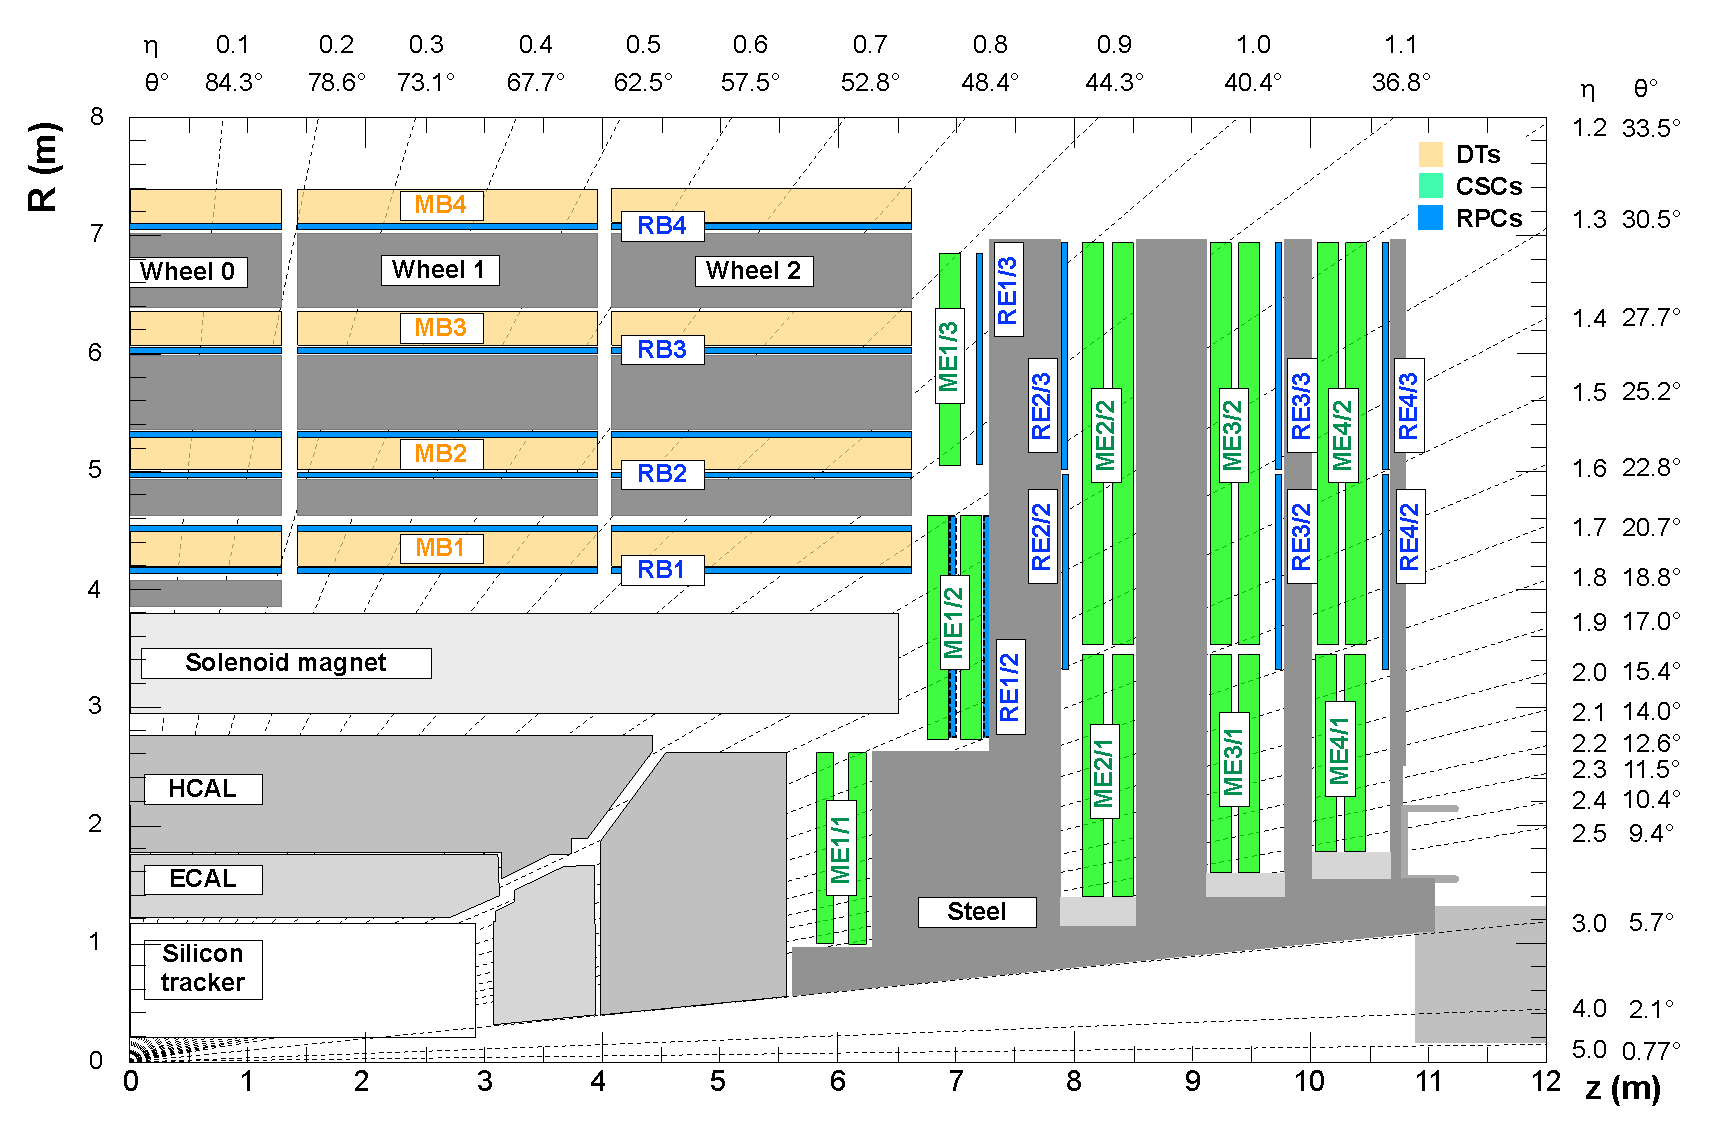
\includegraphics[width=.8\linewidth]{tex/Part2/fig/DT/cms_upg_o_g_b_ni_130619.pdf}
\caption{
  Longitudinal view showing one quarter of the CMS muon detector system.
  The DT chambers are shown in orange color in the Barrel region. 
  The numbering scheme for the chambers consists of a wheel number (YB=0,$\pm$1,$\pm$2), a radial station number (MB1-MB4), and phi sector (S1-S12).
}
\label{fig:DT_layout}
\end{figure}


\section{Data Acquisition}

The DT trigger and readout electronics will be completely replaced by an upgraded system for Phase-2 in order to cope with the higher data rates and L1 trigger demands.
Figure~\ref{fig:DT_DAQ2} shows a comparison of the current components of the DT back end and the new architecture for Phase-2 \cite{CERN-LHCC-2017-012}.
In the Phase-2 design, the front-end electronics are upgraded with On-Board Electronics for DT (OBDT) hosting a PolarFire FPGA.
The data, including the full collection of DT and RPC hits, will be continously streamed via high speed optical
links to the back-end Barrel Layer 1 processor boards (L1 processors) where the trigger primitives are reconstructed.
The L1 processors will consist of ATCA boards capable of processing full DT phi sectors (60),
and will allow for significant improvements in the trigger primitive reconstruction including bunch crossing identification
through improved timing resolution as well as improved spatial resolution close to the performance available offline in the current system. 


For the online luminosity measurement, the BRIL Histogramming firmware described in Chapter~\ref{ch:BRILDAQ}
operating in synchronous mode will be installed as part of the back-end Layer 1 processor firmware.
This histogramming module will access and count the list of trigger primitives in parallel to the CMS L1 trigger stream
and produce a histogram with counts per bunch crossing (3564 bins) at approximately 1 second integration intervals.
Based on the expected number of trigger primitive counts per bunch crossing, the required memory per histogram is estimated at 28 Kb,
requiring a minimal amount of the L1 processor resources. 
The histograms  will be transferred to the BRILDAQ system as part of the IPBus network traffic used for the slow control the DT back-end.
The total data rate expected for the DT luminometer (250 histograms) at the BRILDAQ end is aproximately 7.1 Mbps.
As for the other luminometers, the individual histograms will be merged inside the BRILDAQ accounting for possible background subtraction and filtering of any misbehaving chambers.
The DT chambers should provide valid data as long as the system has been properly configured at least once after LHC RAMP UP phase and the DT HV is ON, which is done at the SQUEEZE stage.
A proper bunch crossing and lumi nible signal should be received, which currently is insured at the DAQ configured state.
The DT system  has  a large redundancy and an electronics system designed with large granularity that remains unaffected by the failure of any single component, having provided a very stable response during operations in Run 1 and 2.
 

A demonstrator of the DT Phase-2 electronics has been installed in one sector (YB+2, S12) to take data during LS2 and Run 3.
For Run 3, a total of 13 OBDT's already installed in LS2 in the four MB stations will be operated with a dual readout using both OBDT's and legacy electronics (legacy mincrates in MB1 and MB2).
A back-end prototype (AB7) based on legacy TwinMux boards is currently used for event matching and trigger primitive generation.
Since 2020, a test version of the BRIL Histogramming firmware has been installed in the AB7 back end and is expected to record data during Run 3.




\begin{figure}[hbtp]
\centering
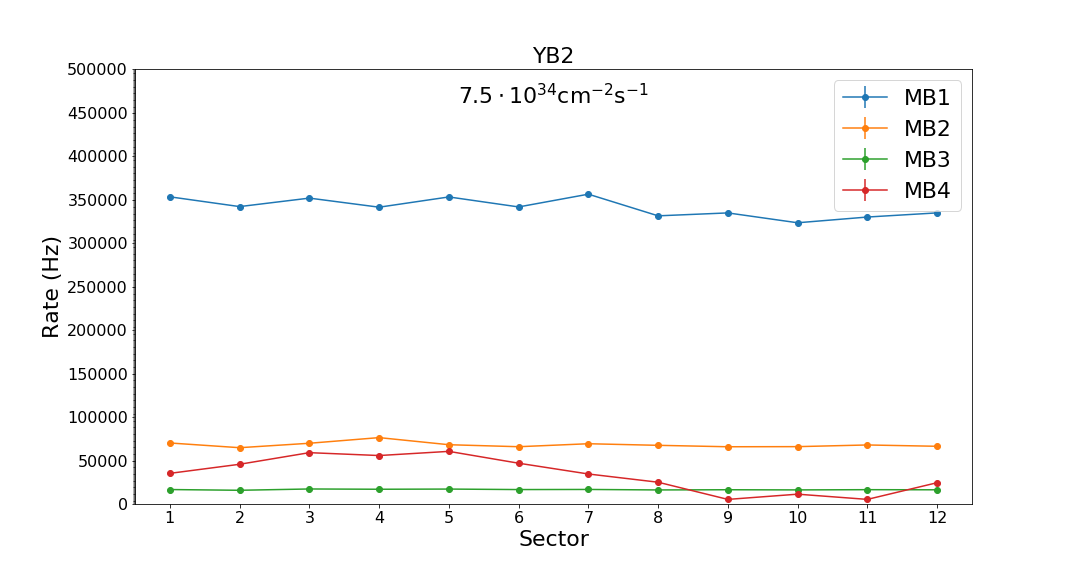
\includegraphics[width=.8\linewidth]{tex/Part2/fig/DT/YB2.png}
\caption{L1 trigger primitive rates expected for HL-LHC instantenous luminosity conditions for the DT chambers in the wheel YB+2.} 
\label{fig:DT_rates}
\end{figure}

\begin{figure}[hbtp]
\centering
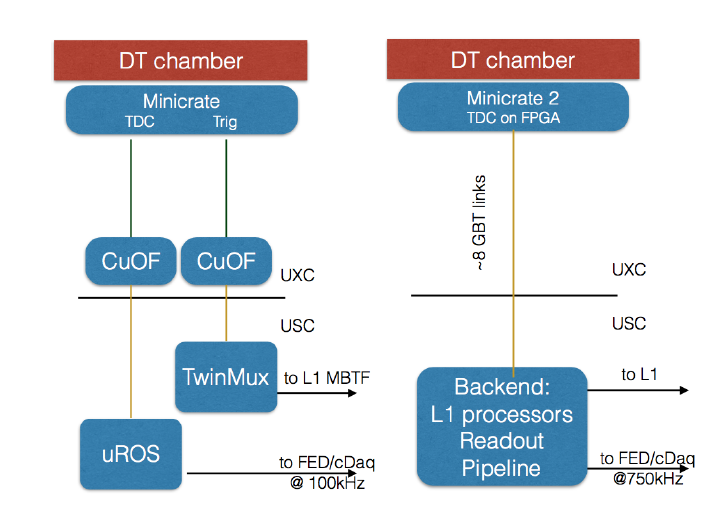
\includegraphics[width=.7\linewidth]{tex/Part2/fig/DT/DT-DAQ-Phase1_vs_Phase2.png}
\caption{
 Current partition of the DT trigger and readout electronics (left) and Phase-2 upgrade design (right) using On-Board Electronics for DT (OBDT).
  The muon trigger primitives will be produced by the L1 processors in the new scheme and not inside the Minicrate ASIC�s as in the present system.
}   
\label{fig:DT_DAQ2}
\end{figure}


\section{Expected Performance}

Despite the increased particle rates at the HL-LHC conditions, the expected hit occupancy for the DT chambers will remain low at about 50 Hz cm$^{-2}$
and the maximum trigger primitive rate per chamber will be below 500 kHz.
At these rates the counting of trigger primitives should remain linear up to high pileup, a necesary property for precision luminosity measurement.
Figure~\ref{fig:DT_linearity} shows the dependence of the total DT trigger primitive rate (using all MB1, MB2, and MB3 stations) on the instantenous luminosity observed in Run 2 data up to about $2\times10^{32}$ cm$^{-2}$ s$^{-1}$.
Up to this luminosity, no systematic deviation from linearity is observed when compared to the HFOC luminometer despite no background corrections have been applied to the DT trigger primitive rates.


Another important aspect is the statistical precision during normal Physics running as well as during the vdM scans used to obtain the calibration constant.
To estimate the statistical precision we use the trigger primitive rates previously extrapolated to the HL-LHC luminosity conditions.
Excluding the MB4 station, the total orbit integrated rate expected is $\sim$17 MHz at $7.5\times10^{34}$ cm$^{-2}$ s$^{-1}$;
this corresponds to about 0.61 trigger primitives per bunch crossing for Physics and 0.00153 per bunch crossing for vdM conditions.    
For the online luminosity measurement, using one colliding bunch and 1 s integration period for Physics (30 s for vdM),
the statistical precision expected is 1.2\% (4.4\%).
During Physics conditions the expected statistical precision meets the requirement of 2\%, while for vdM a precision of 0.36\%,  meeting the requirements for the calibration constant of 1\%, will be obtained  after combining all colliding bunches, 150 assummed here.
The final precision of this luminometer will depend additionally on the ability to handle any backgrounds and keep a stable operation of the detectors and DAQ over entire run periods.


\begin{figure}[hbtp]
\centering
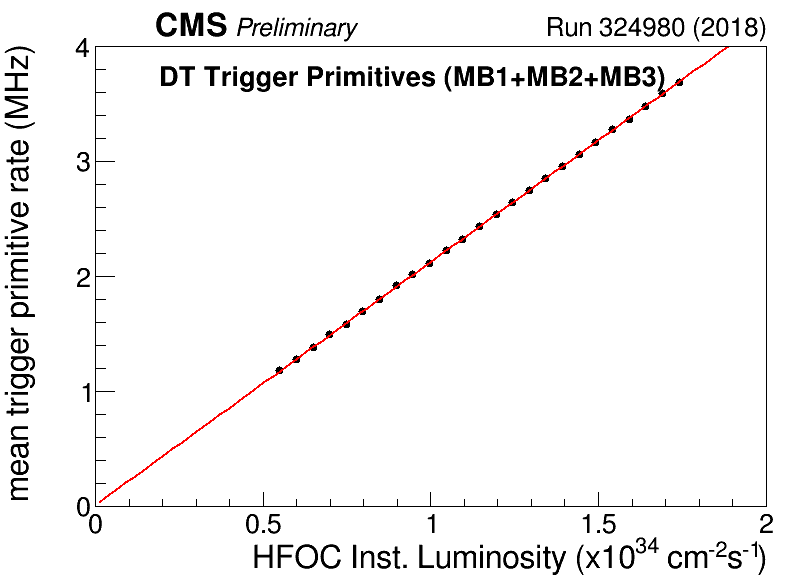
\includegraphics[width=.49\linewidth]{tex/Part2/fig/DT/DT_Trigger_Primitives__MB1pMB2pMB3__Linearity.png}
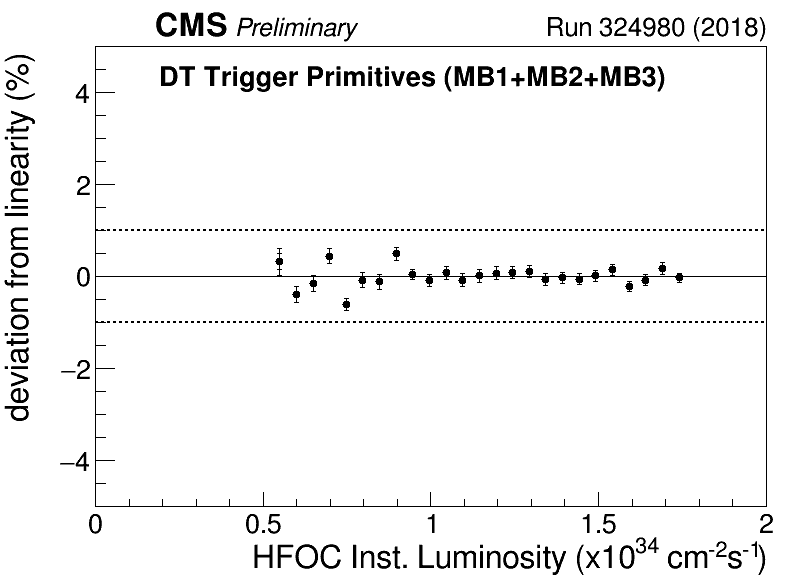
\includegraphics[width=.49\linewidth]{tex/Part2/fig/DT/DT_Trigger_Primitives__MB1pMB2pMB3__Linearity_residuals.png}
\caption{Total DT trigger primitive rate from the MB1, MB2, and MB3 stations as a function of the instantenous luminosity measured by the HFOC luminometer in one Physics run during 2018
(left) and relative deviations from the linear fit (right).} 
\label{fig:DT_linearity}
\end{figure}




%%
%%For muon trigger stub counting, the use of trigger scouting methods prototyped at the end of Run 2
%%will allow per-bunch emittance scan analysis as well as luminosity measurement in physics conditions.
%%Muon trigger stub counting in Run 2 was orbit-integrated at per-LS frequency in real time;
%%using trigger scouting online bunch-by-bunch measurement at 4LN frequency is targeted in Run 3.
%%
%%It is also foreseen to ... expand the muon DT and resistive plate chamber (RPC) functionality to provide bunch-by-bunch
%%trigger primitives instead of a value integrated over a complete orbit.
%% orbit-integrated DT muon stub counting in Run 2 was available in real time at LS frequency.
%%
%%In Run 2, techniques like the DT muon trigger stub counting and the RAMSES radiation monitoring have proven
%%to be useful for stability and linearity studies, and they are planned to be exploited also in Phase-2.
%%To alleviate some of the limitations and allow per-bunch measurements, there is a requirement for Phase-2
%%for the upgrade of the muon counting for luminosity to have a 40MHz readout, as described in Section 7.4.2.
%%
%%In Run 2, counting of track candidates in the barrel muon systems has been shown to have good
%%linearity and can be used for stability and linearity monitoring of other luminometers. The CMS
%%DT chambers are installed in the return barrel yoke and provide muon tracking and triggering
%%for CMS physics operation. The observable used in both Run 1 and Run 2 was the barrel sorter
%%rate from the barrel muon track finder (BMTF), which counts muon track candidates with lumi
%%section granularity, but integrated over all bunches in the orbit. The statistical uncertainty
%%in the orbit-integrated rates at a luminosity of 2 x 1034 cm2 s1 is 0.2\%.
%% Assuming a fill of 2544 equally populated colliding bunches, the statistical uncertainty per BX would be 12%.
%% A naive extrapolation to a total luminosity of 51034 cm2 s1 for HL-LHC yields a statistical
%% uncertainty per BX of 8%.
%%
%%Drift tube muon system: As mentioned, the current implementation of DT luminosity
%%is extremely useful, but it does not provide the necessary statistical precision and
%%time granularity to meet Phase-2 requirements. Thus the rates and statistical uncertainties
%%achievable with different levels of muon trigger objects need to be studied
%%in detail to identify the most suitable one for a 40MHz precision online measurement.
%%The possibility of using the DT back-end electronics for dedicated luminosity
%%processing during Run 3 should be investigated.
%%

%\begin{figure}[hbtp]
%\centering
%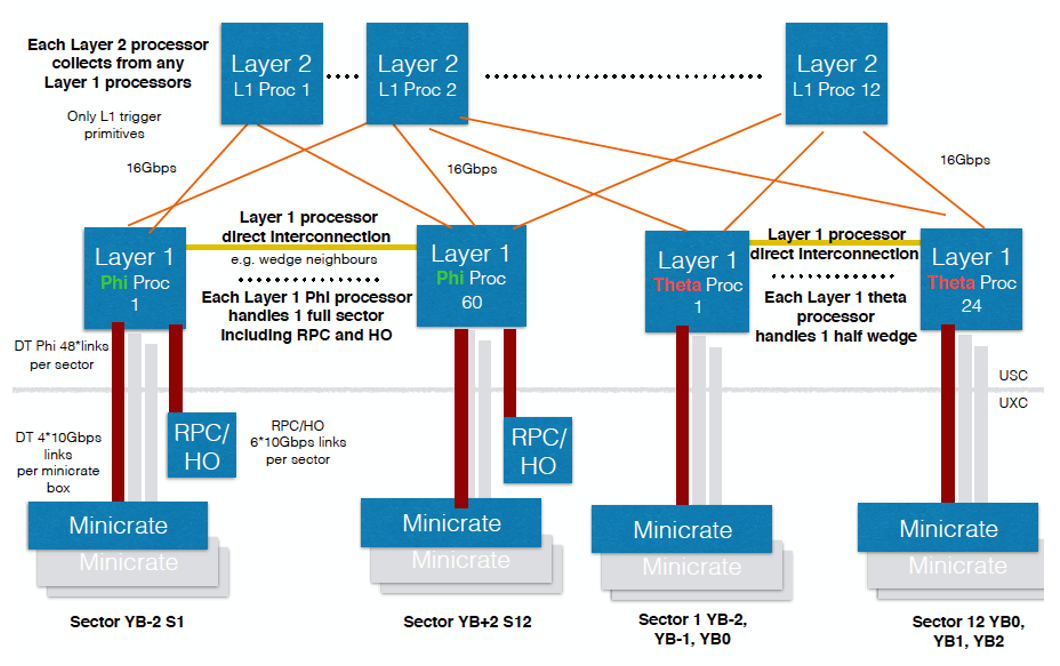
\includegraphics[width=.65\linewidth]{tex/Part2/fig/DT/DT-DAQoverview.png}
%\caption{Design  of the Muon DAQ system architecture for Phase II showing the different layers where the L1 trigger objects are generated. In  this layout the DT trigger primitives are generated in the Layer 1 of the backend.}   
%\label{fig:DT_DAQ}
%\end{figure}
